\documentclass[12pt,a4paper]{article}

% =================================================
% LANGUE ET TYPOGRAPHIE
% =================================================
\usepackage[T1]{fontenc}
\usepackage[utf8]{inputenc}
\usepackage[french]{babel}
\usepackage{lmodern}
\usepackage{microtype}

% =================================================
% MISE EN PAGE
% =================================================
\usepackage[
    a4paper,
    top=2.7cm,
    bottom=2.5cm,
    left=2.7cm,
    right=2.7cm,
    headheight=16pt
]{geometry}

\usepackage{setspace}
\setstretch{1.15}
\setlength{\parindent}{0pt}
\setlength{\parskip}{6pt}

% =================================================
% COULEURS ET TITRES
% =================================================
\usepackage{xcolor}
\definecolor{bleufonce}{HTML}{17365D}
\definecolor{bleuclair}{HTML}{DCE6F1}
\definecolor{gris}{HTML}{313131}

\usepackage{titlesec}

\titleformat{\section}
  {\Large\bfseries\color{bleufonce}}
  {\thesection.}{0.7em}{}
  [\vspace{3pt}\color{bleuclair}\titlerule]

\titleformat{\subsection}
  {\large\bfseries\color{bleufonce}}
  {\thesubsection}{0.7em}{}

\titlespacing*{\section}{0pt}{24pt}{12pt}
\titlespacing*{\subsection}{0pt}{16pt}{8pt}

% =================================================
% IMAGES ET LIENS
% =================================================
\usepackage{graphicx}
\usepackage{float}
\usepackage{hyperref}

\hypersetup{
    colorlinks=true,
    linkcolor=bleufonce,
    urlcolor=bleufonce,
    pdftitle={Rapport de projet C++},
    pdfauthor={Raïan CHOUIREF et Dorian LEON FERNANDES}
}

% =================================================
% EN-TÊTES ET PIEDS DE PAGE
% =================================================
\usepackage{fancyhdr}

\pagestyle{fancy}
\fancyhf{}

\fancyhead[L]{\small\textcolor{gris}{Rapport de projet C++}}
\fancyhead[R]{\small\textcolor{gris}{Programmation et géométrie}}

\fancyfoot[L]{\small\textcolor{gris}{Raïan CHOUIREF -- Dorian LEON FERNANDES}}
\fancyfoot[R]{\small\textcolor{gris}{Page \thepage}}

\renewcommand{\headrulewidth}{0.4pt}
\renewcommand{\footrulewidth}{0.4pt}

% =================================================
% SOMMAIRE
% =================================================
\usepackage{tocloft}

\renewcommand{\contentsname}{Sommaire}
\renewcommand{\cftsecfont}{\bfseries\color{bleufonce}}
\renewcommand{\cftsecpagefont}{\bfseries\color{bleufonce}}
\setlength{\cftbeforesecskip}{8pt}

% =================================================
% DOCUMENT
% =================================================
\begin{document}

% =================================================
% PAGE DE GARDE
% =================================================
\begin{titlepage}
    \thispagestyle{empty}

    \centering

    \vspace*{2cm}

    {\Large\textcolor{gris}{RAPPORT DE PROJET}\par}

    \vspace{1.5cm}

    {\color{bleufonce}\rule{\textwidth}{1.5pt}\par}

    \vspace{0.7cm}

    {\Huge\bfseries Rapport C++\par}

    \vspace{0.5cm}

    {\Large\textcolor{gris}{Structures de données et affichage 3D}\par}

    \vspace{0.7cm}

    {\color{bleufonce}\rule{\textwidth}{1.5pt}\par}

    \vspace{2.5cm}

    {\large\textbf{Réalisé par}\par}

    \vspace{0.5cm}

    {\Large Raïan CHOUIREF\par}
    \vspace{0.2cm}
    {\Large Dorian LEON FERNANDES\par}

    \vfill

    % Pour ajouter un logo, décommente les lignes suivantes
    % et remplace logo.png par le nom de ton image.
    %
    % \includegraphics[width=3cm]{logo.png}
    % \vspace{1cm}

    {\large Année universitaire : \rule{4cm}{0.4pt}\par}

    \vspace{0.5cm}

    {\large \today\par}

    \vspace{1cm}

\end{titlepage}

% =================================================
% SOMMAIRE
% =================================================
\pagenumbering{roman}

\tableofcontents

\newpage

% =================================================
% CONTENU DU RAPPORT
% =================================================
\pagenumbering{arabic}

\section{Introduction}

% Présenter le sujet, les objectifs et les grandes étapes
% du projet.

\vspace{4cm}

\section{Problème}

% Expliquer le problème étudié et les objectifs à atteindre.

\vspace{4cm}

\section{Contexte du projet}

% Présenter le contexte, les outils utilisés et les contraintes.

\vspace{4cm}

\newpage

\section{UML}

% Ajouter le diagramme UML et expliquer les classes,
% leurs attributs, leurs méthodes et leurs relations.

% Exemple pour insérer un diagramme :
% \begin{figure}[H]
%     \centering
%     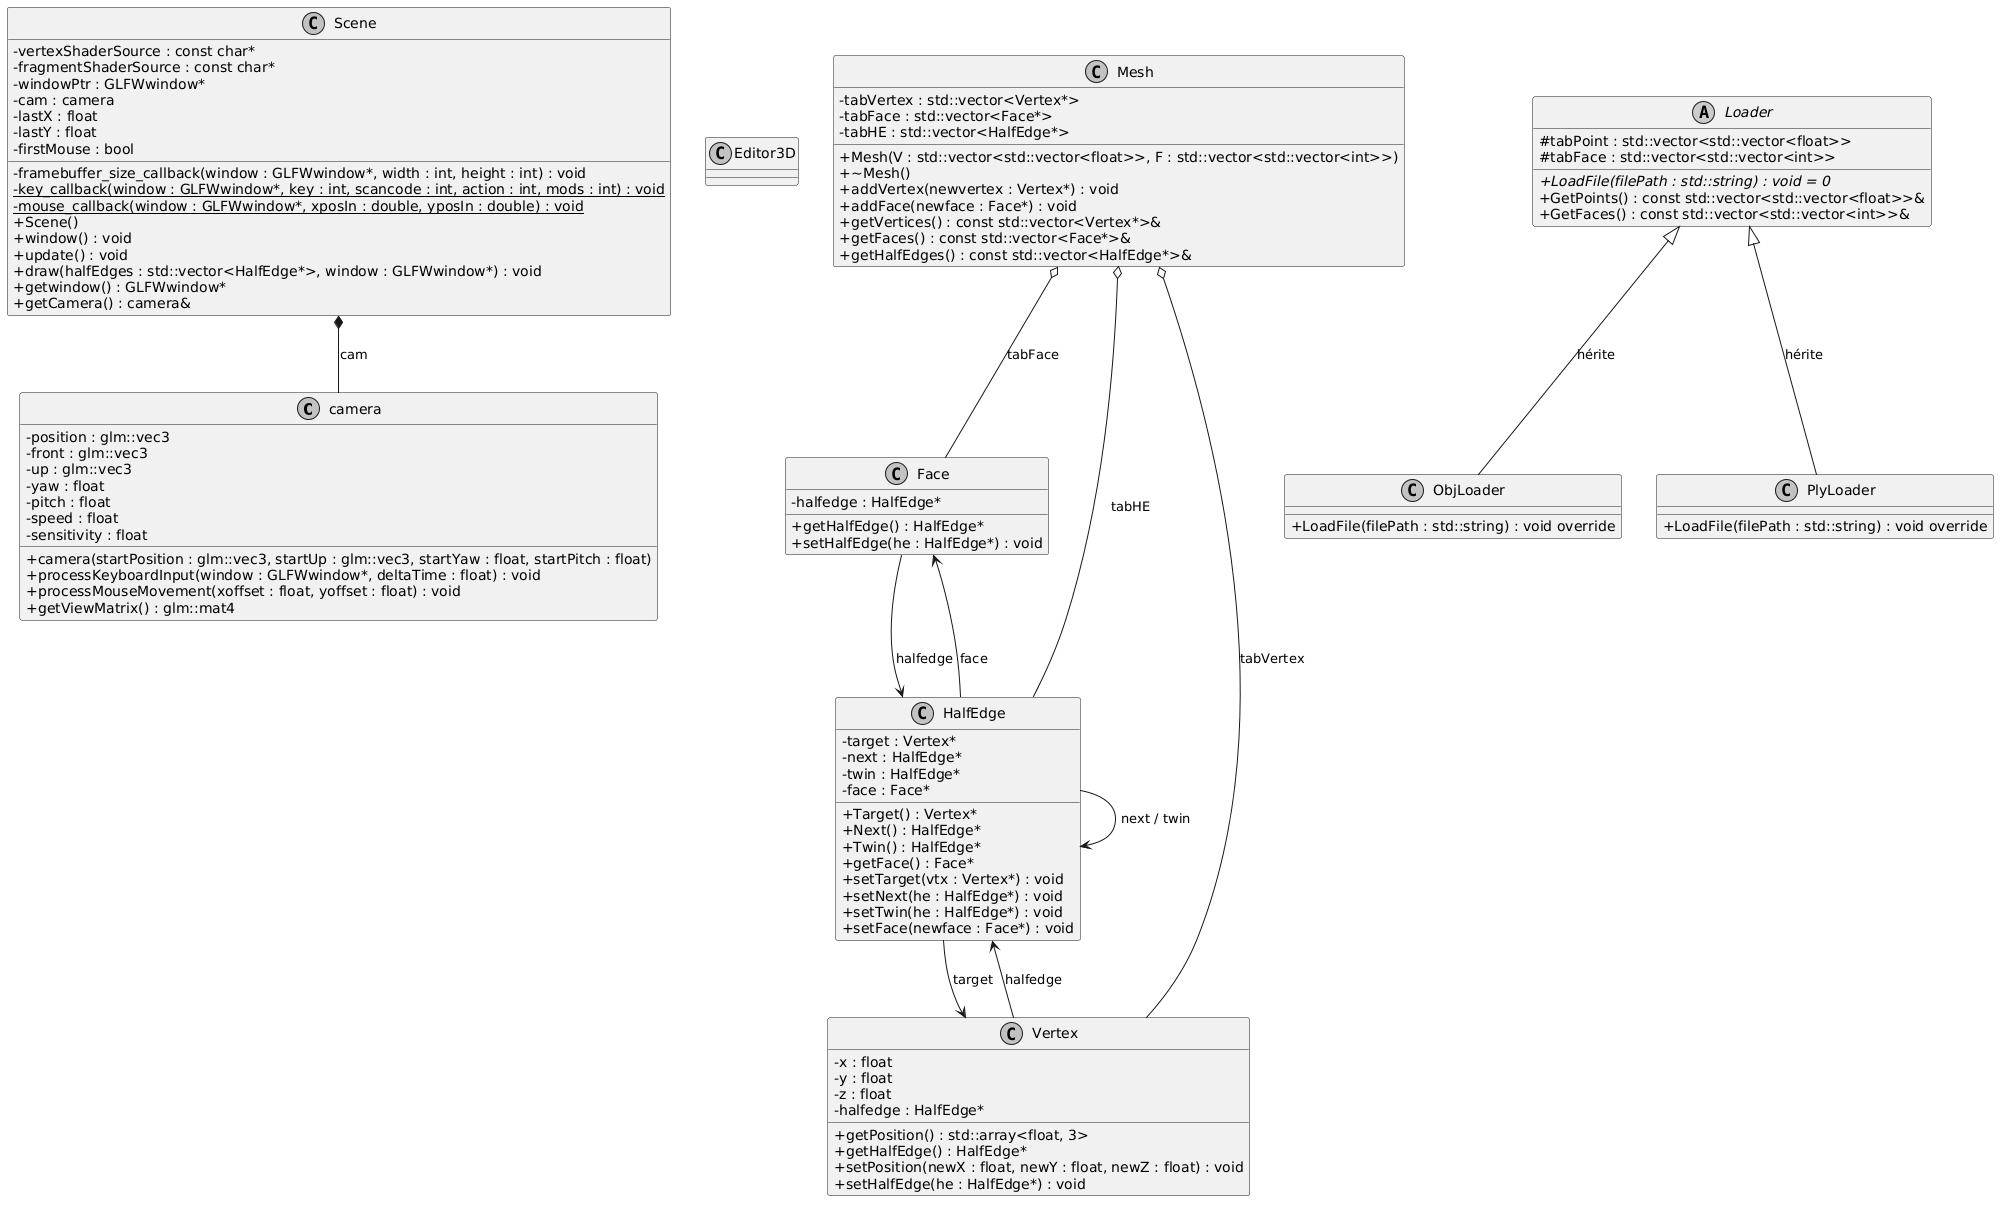
\includegraphics[width=0.85\textwidth]{uml.png}
%     \caption{Diagramme UML du projet}
%     \label{fig:uml}
% \end{figure}

\vspace{4cm}

\section{Halfedge}

% Expliquer la structure Halfedge, son fonctionnement,
% les liens entre les éléments et son utilisation dans le projet.

\vspace{4cm}

\newpage

\section{Affichage}

% Présenter le système d'affichage, OpenGL, le rendu
% graphique et les interactions éventuelles.

\vspace{4cm}

\section{Loader}

% Expliquer le chargement des fichiers .PLY et .OBJ,
% leur lecture et la conversion des données en structures
% utilisables par le programme.

\vspace{4cm}

% =================================================
% CONCLUSION (À COMPLÉTER SI NÉCESSAIRE)
% =================================================
\newpage

\section{Conclusion}

% Faire le bilan du projet, présenter les difficultés
% rencontrées et les améliorations possibles.

\vspace{5cm}

\end{document}